\documentclass[11pt,a4paper]{article}
\usepackage{epsfig}
\usepackage{multicol}
\usepackage[margin=0.7in]{geometry}
%\usepackage[dvipsnames]{xcolor}
\usepackage{textcomp}
\usepackage{graphicx}
\usepackage{caption}
\usepackage{subcaption}
\usepackage{amsmath}
\usepackage{tcolorbox}
\usepackage{pict2e}
\usepackage{tikz}

\begin{document}
\section{Introduction}
%cancer
Cancer is now well established as a family of diseases whose development is considered to be determined by three main factors: Mechanics, Immune system and Metabolism. Analysis of physiological parameters on live subjects, or adapted \textit{in vitro} models have consistently demonstrated that cancer initiation and progression can be be robustly correlated to notable change in at least one of these aspects. The mechanical properties of cells and tissues evolve, with a general trend being that cells become more deformable while tissues become more rigid due to increased extracellular matrix production.\cite{Chin2016} In terms of the immune system, many complex responses invovling deregulation of immune response have been observed.\cite{Pardoll2015} Moreover, there are instances where immune cells can be recruited by adjacent cancer cells and effectively promote tumor growth by affecting the surrounding healthy tissue.\cite{Gonzalez2018} Metabolic reprogramming during cancer progression generally involves increased resistance to nutrient scarcity along with a increased ability to rely on multiple substrates for growth and survival. In several cancer types, experiments have suggested that metabolic adaptation is linked to hypoxia, notably through the action of Hypoxia-Inducible-Factors (HIF).\cite{Rakotomalala2021}

%hypoxia
The physiological impacts of hypoxia have long been studied in various cancer cell lines. From a regulatory point of view, the involvement of Hypoxia-inducible factors (HIF), proteins regulating transcription and responding to low oxygen levels is now well established.\cite{Strickland2017}\cite{Chen2021} However, the dynamics of different isoforms and their link with other physiological markers are difficult to decipher and are actively studied to this day. One of the reasons for this is the variability of observed responses. Some cell lines have demonstrated constitutive hypoxic response even when well oxygenated.\cite{Aebersold2001} Several cancer cell lines exhibit resistance to hypoxic conditions, some surviving for weeks at oxygen level below 1\% \cite{McKeown2014}. This state of facts calls for more qualitative and quantitative data on the variety and details of hypoxia responses in different cell lines.

%Why studying hypoxia is difficult
Relevant study of hypoxia on \textit{in vitro} models can be difficult. As suggested in several studies, oxygen levels in normal incubators tend to be higher than even" physoxic" levels near capillaries and blood vessels in healthy tissue, which are reportedly ranging from  3 to 7.4 \%.\cite{McKeown2014} If one wants to account for the possible organ geometries, variations in tissue diffusion and the possible impact of tumor development on all the previous parameters, reproducing tissue structure, at least to a degree, is a promising pathway to relevance and reproduction of biophysical parameters.

%Pediatric glioma and the chip
Pediatric gliomae are among the type of tumors whose development has been linked to hypoxia most notably through the H3K27M histone and the impact of hypoxia on its dynamics.\cite{Rakotomalala2021} The aim to reproduce a relevant metabolic environment for tumor growth has led to the development of a tumor-on-chip model with dimensions compatible with the formation of oxygen gradients and recreating hypoxic growth conditions found \textit{in vivo}.

%why use modelling 
The complex geometry of the system as well as the number or unknown or open parameters in terms of cell metabolic behavior, in general and in the specific context of hypoxic growth would require a high number of experiments to gain insights about the system. In this case, the benefit of integrating \textit{in silico} modelling into this type of studies is two-fold. It can confirm or infirm simple hypotheses about the system and potentially allow the exploration of different parameters and their impact of growth. This study thus focuses on the development of a computational model capturing the main features of growth and oxygen dynamics within the tissue in DMG-on-chip experiments.

\section{The model}
\subsection{Agent-based modelling for cancer studies}
%Cancer and tumor growth
Modelling of tumor growth  and other cancer tissue properties is a research field more than 50 years old and various types of model have been used to capture the main feature of various living systems and their interactions with their surroundings. Different types of models are used to describe processes on different spatial and temporal scales. Systems biology, for example, has used modelling to describe regulatory network and mean-field models have been used to describe tissue-scale growth and response to environment.Use of computational tools to solve the model has progressed along with the available computational power in the last decades, and two great types of model have emerged over the years to capture both cell-level response mechanisms and tissue-scale growth and geometry: continuous model and agent-based models. 

%Continuous models 
Continuous models represent most variables as densities or concentrations which are linked by ordinary differential equations and/or partial differential equations. Cell or tissue response to their environment is then generally encompassed in mathematical functions. Continuous models with few variables do not require the use of computational tools and some of them can even be solved analytically. However, finer modelling and inclusion of coupled can make computational tools necessary to solve the equations. Applications in terms of cancer range from description of bacterial movements to the complex regulatory response of a tissue coupled to growth to spheroid growth or cell migration.\cite{Casciari1992}\cite{Villa2021}\cite{Katsaounis2023}

%Agent-based models
Agent-based models represent cells (or sometimes groups of cells) as individual agents and use algorithmic rules instead of mathematical functions to encode cell behavior and interactions with their environment and one another. In most cancer modelling studies, agent-based models are generally coupled to a set of partial differential equation to describe nutrients of cytokines/chemokines or the evolution of surrounding environment. Agent-based models can be classified into "off-lattice" and "on-lattice" models.\cite{Osborne2017} In "off-lattice" models, the three-dimensional space is represented as triplet of real numbers and cell movement and deformations are calculated by solving Newton's 3rd law. "On-lattice" models represent cells as points on a fixed grid. In general off-lattice model are better at describing phenomenon where stress or any mechanical quantity needs to known quantitatively. On-lattice are simpler and remain useful as long as a coarse discrete description of space does not impact results too negatively.

In this study the characteristics of the system made it possible to use an hybrid on-lattice agent based model which is described herefater.

\subsection{Agent-based modelling for the DMG-on-chip}
%the model
The model used in this study is a hybrid on-lattice agent-based model. This model can be broadly understood as a collection of links and interactions between three main grids : The cellular grid, the nutrient grid and the consumption grid. 

%The cellular grid 
The cellular grid keeps tracks of whether a vertex in the lattice is occupied or not. If it is, then the grid value is set to the index of the cell occupying it. Cells are attributed a unique index when they appear in the model either at initialisation or through mitosis.

%The nutrient grid
The nutrient grid is handled by a finite difference algorithm which update the concentration at every timestep. This grid is also checked whenever cell response to the environment is set to occur. In this case, only oxygen dynamics is modelled as no data on glucose was collected. But addition of glucose would be straightforward if needed.

%The consumption grid
This grid is updated regularly to reflect the evolution of cellular nutrient consumptions rates and the impact of their position on the spatial distribution of nutrients.

%Other data structures
This grid are linked together but also to other important data structures in the model such the cell table, which contains the information of all cells in the model sorted by index. 

%The evolution 
The model is ran minute-by-minute. Every minute, the model checks whether any modification is necessary on the cellular grid. For example, some cells migrate, divide or commit to death, then the three grids are updated to reflect that change. Once the cellular checks are run, the nutrient grid is updated by running the finite difference algorithm for a minute.

%Grid structure 
The chosen model structure has the advantage of providing vertex-to-vertex match between all three grids. This avoids any interpolation or calculation of spatial coordinates which reduces computational work and is conducive to parallelization.\\

\begin{figure}[ht]
\begin{center}
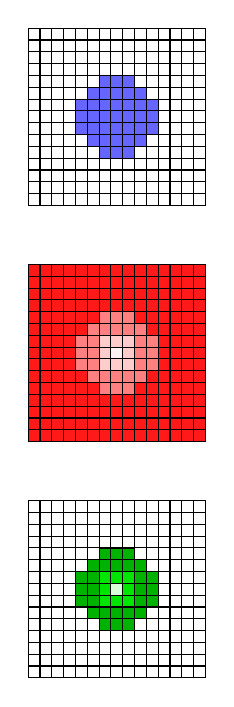
\begin{tikzpicture}
\begin{scope}[scale=1.5]
	\draw (0,0) grid[step=0.1] (1.5,1.5) rectangle (0,0);
	
    \draw[fill=blue!60!white] (0.5,0.5) grid[step=0.1] (1.0,1.0) rectangle (0.5,0.5);
    \draw[fill=blue!60!white] (0.4,0.6) grid[step=0.1] (1.1,0.9) rectangle (0.4,0.6);
 	\draw[fill=blue!60!white] (0.6,0.4) grid[step=0.1] (0.9,1.1) rectangle (0.6,0.4);
 	%\draw[->]
 	
 	\begin{scope}[yshift=-2cm]
 		\draw[fill=red!90!white] (0,0) grid[step=0.1] (1.5,1.5) rectangle (0,0);
	
    	\draw[fill=red!50!white] (0.5,0.5) grid[step=0.1] (1.0,1.0) rectangle (0.5,0.5);
   		\draw[fill=red!50!white] (0.4,0.6) grid[step=0.1] (1.1,0.9) rectangle (0.4,0.6);
 		\draw[fill=red!50!white] (0.6,0.4) grid[step=0.1] (0.9,1.1) rectangle (0.6,0.4);
 		\draw[fill=red!20!white] (0.6,0.6) grid[step=0.1] (0.9,0.9) rectangle (0.6,0.6);
 		\draw[fill=red!5!white] (0.7,0.7) grid[step=0.1] (0.8,0.8) rectangle (0.7,0.7);
 	\end{scope}
 	
 	\begin{scope}[yshift=-4cm]
 	 	\draw (0,0) grid[step=0.1] (1.5,1.5) rectangle (0,0);
	
    	\draw[fill=green!70!black] (0.5,0.5) grid[step=0.1] (1.0,1.0) rectangle (0.5,0.5);
    	\draw[fill=green!70!black] (0.4,0.6) grid[step=0.1] (1.1,0.9) rectangle (0.4,0.6);
 		\draw[fill=green!70!black] (0.6,0.4) grid[step=0.1] (0.9,1.1) rectangle (0.6,0.4);
 		\draw[fill=green!90!black] (0.6,0.6) grid[step=0.1] (0.9,0.9) rectangle (0.6,0.6);
 		\draw[fill=green!15!white] (0.7,0.7) grid[step=0.1] (0.8,0.8) rectangle (0.7,0.7);
 	\end{scope}
\end{scope}
\end{tikzpicture}
\caption{Schematic representation of the data structure of the simulation\label{structure_model}}
\end{center}
\end{figure}

In the following the model is presented in more detail.

\subsection{DMG-on-chip build-up geometry}
The DMG-on-Chip (DoC) geometry is as follows: a 13mm-diameter cylindrical well is cut into a PolyDiMethylSiloxane (PDMS) mold. Two side inlets that are directly connected to the circular part. The inlet are the 3 mm-wide and have rectangular geometry. The PDMS mold is placed on a lower glass cover slip and is 750 \textmu m-thick. The PDMS mold lateral dimensions are 4 $\times$ 2 mm². The overall layout is shown in figure \ref{drawing}

\begin{figure}[ht]
\begin{center}
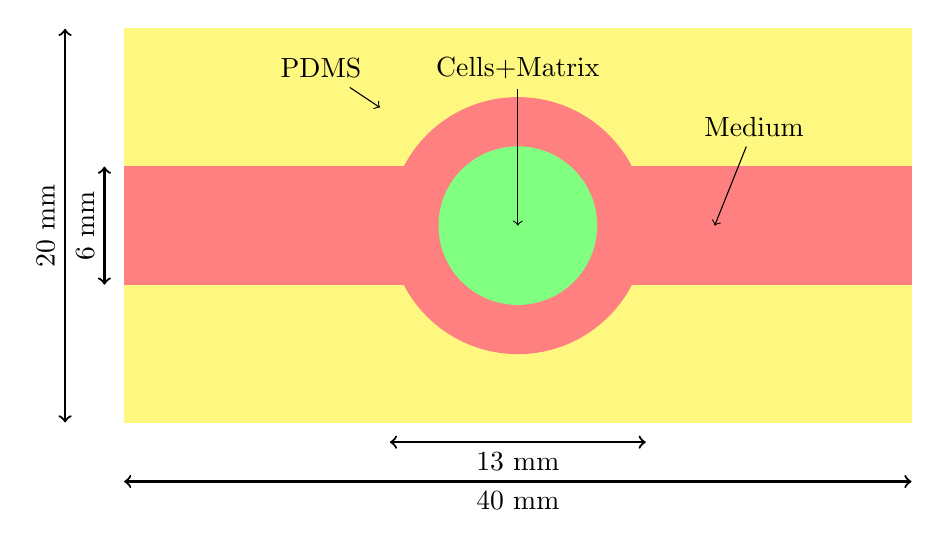
\begin{tikzpicture}
\begin{scope}[scale=0.25]
\draw[color=yellow!50!white , fill=yellow!50!white] (0,0) rectangle (40,20);
\draw[color=red!50!white,fill=red!50!white] (40/2,20/2) circle (6.5);
\draw[color=red!50!white,fill=red!50!white] (0,20/2-3) rectangle (40,20/2+3);
\draw[color=green!50!white,fill=green!50!white] (40/2,20/2) circle (4);

\node (P) at (10,18) {PDMS};
\node (C) at (20,18) {Cells+Matrix};
\node (M) at (32,15) {Medium};

\draw[->] (P)--(13,16);
\draw[->] (C)--(20,10);
\draw[->] (M)--(30,10);

\draw[thick,<->](-3,0)--(-3,20) node[midway,above,sloped]{20 mm};
\draw[thick,<->](-1,20/2-3)--(-1,20/2+3) node[midway,above,sloped]{6 mm};
\draw[thick,<->](0,-3)--(40,-3) node[midway,below,sloped]{40 mm};
\draw[thick,<->](40/2-6.5,-1)--(40/2+6.5,-1) node[midway,below,sloped]{13 mm};
\end{scope}
\end{tikzpicture}
\caption{Schematic representation of the layout of the system\label{drawing}}
\end{center}
\end{figure}

%The cell pellet 
The cell pellet, made of a mixture of cell, matrigel, hyaluronan and reticulant is poured into the well to form a circular pellet near the center of the circular well. The pellet is then left to reticulate and form an assembly of cells embedded in 3D cellular matrix. This pouring and reticulation process means the exact diameter of the pellet cannot be controlled. Usual values for experiments were between 9 and 10 mm.

%finishing the setup
Fresh culture medium is then poured in the remaining spaces of the PDMS mold to supply the 3D culture with nutrients. This way, the nutrients and oxygen in the medium are supplied radially to the cells through the matrix. Once the pellet and medium are in place, an upper coverslip is placed on top of the system. The upper coverslip is placed in a perpendicular arrangement comapred to the first one in order to keep part of the inlets uncovered. This ensures that oxygen renewal occurs only at the end of each inlet and that the nutrient and oxygen supply is indeed radial. Once everything is in place, the system is placed in culture conditions and monitored for the next 24 to 48 hours.


\subsection{Oxygen dynamics}
The oxygen dynamics is modelled with the following reaction diffusion equation which is commonly used to model nutrient dynamics in hybrid agent-based models.\cite{Mao2018}\cite{Kempf2005}\cite{Bull2020}. In our case, the reaction-diffusion equation is written as:

\begin{align}
\label{eqn:O} \frac{d [O]}{d t} = \overrightarrow{\nabla} (D_O \cdot \overrightarrow{\nabla} [O]) - k_O \frac{[O]}{[O] + O_0}  
\end{align}

With $[O]$ the oxygen concentration, $D_O$ the diffusion coefficient of oxygen and $k_O$ the maximum oxygen consumption rate (OCR). The equation as written above holds for a given phase. Physically speaking, the model comprises three areas which are delineated and color-coded in figure \ref{drawing}, in the following the physical description of each phase in the model and its relation to oxygen dynamics will be detailed.

%culture medium
Culture medium is generally modelled as 37°C water in modelling studies focused on cancer.\cite{Mao2018}\cite{Kempf2005}\cite{Bull2020}\cite{Jagiella2016} However, the amount of dissolved species in standard culture medium formulations has led some researchers to questioning that assumption. However, literature and experiments on this subject remain scarce at the time of this writing. But one study on the subject did demonstrate potentially significant effect of dissolved species such as glucose, sodium chloride and anionic surfactants on the measurable oxygen diffusion coefficient.\cite{Jamongwong2010} In standard culture medium, glucose mass concentration generally ranges between 0 and 4.5 g/L. In this concentration range, the study demonstrates that dissolved glucose does not signficantly impact oxygen diffusion coefficient. In terms of salts, the concentration of NaCl is varied between 0 and 100  g/L and is shown to have a significant effect on oxygen diffusion coefficient. A typical culture medium formulation includes roughly 11 g/L of inorganic salts including 6.4 g/L of NaCl. According to the measurement of Jamongwong et al., this may result in a 25 \% decrease of the diffusion coefficient compared to pure water. It would therefore be reasonable to apply a corrective factor to the 37°C value for water. Moreover, the presence of anionic surfactants even in low amount, impacts the diffusion coefficient as well, but none of the vitamins present in studied formulations used as reference that might be an anionic surfactant is present in sufficient amount to be within the range shown to impact diffusion coefficient. Interestingly, a study by Figueieredo and colleagues measured almost identical values for the oxygen diffusion coefficient of water and DMEM.\cite{Figueiredo2018} Therefore, the retained diffusion value for oxygen is that of 37°C reduced by 25\% due to salt which results in the value range used in the model being 135000-180000 \textmu m$^2$/min.

%The pellet
The pellet, consists of a mixture of matrigel and hyaluronic acid saturated with culture medium and containing cells. A study by Colom and colleagues contains experimental data on oxygen diffusion in cellular and acellular gels compared to water.\cite{Colom2014} One of the tested gels was partially composed of matrigel. The oxygen diffusion coefficient measured on matrigel was a 40\% reduction compared to the value found in water. Another study by Figueiredo and colleagues also provides diffusion oxygen coefficient for hydrogels and several biological scaffolds, and some are as low as 15 \% of the value found in water.\cite{Figueiredo2018} The range of value retained for culture medium in this modelling case being between 135000-180000 \textmu m$^2$/min, a realistic range for acellular matrix would be 20000-110000 \textmu m$^2$/min. It also mentioned that cellularized matrix exhibit a diffusion value 40 \% lower than the cellularized matrix, meaning a convincing range for cellularized matrix would be between 10000 and 66000 \textmu m$^2$/min.

%PDMS
Reticulated PDMS is permeable to oxygen. This means that in order to fully model the oxygen dynamics, it is necessary to include the PDMS mold in the model. Reticulated PDMS can be described as a tortuous gas phase. A survey of the available literature on diffusion oxygen coefficient in oxygen yielded values ranging from 100000 \textmu m$^2$/min to 540000 \textmu m$^2$/min in various measurement and molecular dynamics studies.\cite{Ullal2014}\cite{Sudibjo2011}\cite{Park2006}\cite{Ziomek1991}\cite{KimM2013}.[improve with information on PDMS]

Since PDMS is described as a gas phase and the medium is described as a liquid phase, the transfer between the PDMS gas phase and the adjacent medium liquid phase needs to be modelled as well. To achieve that, the two-film theory is used.\cite{Doran2012} Since the model focuses on oxygen in aqueous solution , the following formula can be applied at the interface :
\begin{align}
\label{eqn:2FT} J_{O2} =  k_L a([O]_{eq}-[O]) 
\end{align}
with $J_{O2}$ the volumetric mass transfer in mol/m$^3$/s, $k_L$ the liquid mass transfer coefficient in m/s, $a$ the area of the interface and $[O]$ the oxygen concentration in the liquid. $[O]_{eq}$ is given by the following equation:
\begin{align}
\label{eqn:HO} [O]_{eq} =  [O]_{PDMS}H_{cc} 
\end{align}
with $H_{cc}$ the Henry coefficient for oxygen in water and $[O]_{PDMS}$ the concentration in the adjacent PDMS. This expression for the flux is used directly in the diffusion equation. According to the studies of Jamongwong et al, the mass transfer coefficient is also impacted by the salt concentration and temperature. The value at 20°C given by Jamongwong, considering the amount of inorganic salts dissolved in ordinary culture medium is 3.8 $\cdot$ 10$^{-4}$ m/s\cite{Jamongwong2010}. Vogelaar and colleagues have studied the impact of temperature on mass transfer coefficient on oxygen.\cite{Vogelaar2000} The value of the mass transfer coefficient increases by 33 \% when temperature increases from 20°C to 40°C. Therefore, a 33 \% increase to the value given by Jamongwong and colleagues is applied to account for temperature influence. The retained value for $k_L$ is 2.5 $\cdot$ 10$^{-4}$ m/s, which is converted to 18000 µm/min for use in the model. 

The value of the Henry coefficient for oxygen is taken to be 4 $\cdot$ 10 $^{-2}$ after application of Van't Hoff's law to account for the influence of temperature.

\subsubsection{Oxygen Consumption Rate}
Before engaging with quantitative aspects, the definition of oxygen consumption rate is briefly reminded. Cell oxygen consumption is a complex process whose characteristics can vary in time as a function of physical and physiological parameters. In models this process is generally divided into two parts. The physical part and the biological part. The physical part correspond to the quotient of concentration in the Hill function and follows a ligand-receptor model. The maximum value, which occurs for "high" concentrations, can change with environmental conditions, cell cycle phase or if a drug such as Oligomycin-A is administered. What is normally as oxygen consumption rate in studies is the maximum value in normal conditions, often referred to as "basal" OCR. \textbf{[commenter plus précisément]}

%broad view by Wagner and colleagues
A good starting point to discuss oxygen consumption quantitatively is the study of Wagner and colleagues in which they reported on a range of measured oxygen consumption rates on various cell types.\cite{Wagner2011} The reported values for maximum consumption rate range between 10 and 50 amol/cell/s, which corresponds to a range between 0.6 3.0 fmol/min/cell which will be the unit in which other values are ultimately converted

For DIPG cells, in most cases, the average oxygen consumption rate in normal conditions has been measured in monolayers through the use of the Seahorse XF$^{TM}$ kit.\cite{RomeroAgilent} The value reported by Shen and collaborators is 4000 pmol/min/$10^6$ cells. This value is reported for HSJD-DIPG-007 cell line cultured as neurospheres.\cite{Shen2019} In another study by Mbah and collaborators, two models from the HSJD-DIPG-007 and SU-DIPG-XIII cell lines were used: one grown as neurospheres and another cultured as adherent monolayer with serum. The OCR was measured in both cases. For the HSJD-DIPG-007 cell line, the OCR value reported for gliospheres-cultured cells reported is 50 pmol/min/cell.\cite{Mbah2022}

The first comparison that can be made is to the value reported by Shen and collaborators, which is 0.004 pmol/min/cell, and to the range reported by Wagner and colleagues, which converts to a range between 0.0006 and 0.003 pmol/min/cell. This means that a similar method in similar conditions on the same cell line yielded results larger by 4 orders of magnitude. Other values reported for brain tumor cells by Ruas and collaborators are in the range of  to 4800 pmol/min/$10^6$ cells measured in suspension on U87 glioma cells.\cite{Ruas2018} This is much closer to the value of Shen and collaborators. A possible explanation is a conversion error by Mbah and collaborators. If the value reported by Mbah and collaborators is taken not to be 50 pmol/min/cell but 50 pmol/sec/$10^6$ cells then it becomes much closer to the other values. And to further support this point, the results on extracellular acidifcation rate (ECAR) are subject to the same discrepancy and can be corrected in the same way. Now, if the correction is applied to the gliosphere values for HSDJ-DIPG-007, the measured OCR is 50 pmol/s/$10^6$ cells, which corresponds to 0.003 pmol/min/cell, which is much closer to other reported values. 
%, and therefore 0.375 mM/min/cell (assuming a 8 pL cell volume). The same operation for SU-DIPG-XIII yields 0.5 mM/min/cell. So the retained range for the cellular oxygen consumption in normal conditions for proliferating cell is chosen to be between 0.375 and 0.5 mM/min/cell. 

It is however interesting to note that a later study on DIPG cell lines reported an OCR between 200 and 600 pmol/min/cells for SU-DIPG17, which does not seem to match any of the previously reported values.\cite{Shen2024} However, it is reported that they used the Seahorse XF protocol with 24-well plates. According to the supplier, cell number in a plate should be approximately 10$^5$ cells. \textbf{[repréciser le raisonnement ici] }Therefore, reporting 200-600 pmol/min for SU-DIPG17 would correspond to 2000-6000 pmol/min/10$^6$ cells. Comparison data between SU-DIPG17 showed that HSJD-DIPG-007 consume 2.5 times less oxygen in basal respiration compared to the SU-DIPG17, which would lead to approximately 800-2400 pmol/min/10$^6$ cells for HSJD-DIPG007 and 500-1500 pmol/min/10$^6$ cells for HSJD-DIPG0012. Even though it has been possible to reconcile apparently incompatible values with reasonable assumptions, the variablity of values and their reporting by different authors means that maximum basal OCR, like matrix oxygen diffusion coefficient, has a relatively large range on realistic values.

%200 pmol/min -> 600 pmol/min/
%0.24 Mcells at confluence for  24-well plate according to thermofischer 
To summarize the various values will be converted into fmol/min/cells and compiled into  table 
\begin{table}
\begin{center}
\begin{tabular}{ |p{50mm}|p{50mm}|p{15mm} |}
\hline
 \textbf{Cell line}  & \textbf{Basal OCR } & Ref. \\
 \hline
  \hline
 HSJD-DIPG-007 neurospheres w/ Seahorse XF & 4.0 fmol/min/cell & \cite{Shen2019}\\
 \hline 
  HSJD-DIPG-007 gliospheres w/ Seahorse XF & 3.0 fmol/min/cell & \cite{Mbah2022}\\
 \hline 
  HSJD-DIPG-007 monolayers w/ Seahorse XF & 0.8-2.4 fmol/min/cell & \cite{Shen2024}\\
 \hline 
   U87 2D cultures XF & 4.8 fmol/min/cell & \cite{Ruas2018}\\
 \hline 
\end{tabular}
\caption{Values of basal oxygen consumption rate for diffrent cell lines and culture methods\label{tab:ocr}}
\end{center}
\end{table}

An important thing to note is that in the model concentrations are given in millimolars. This means concentration cannot be directly injected into the model and must first  be converted from fmol/min/cell into mM/min. This conversion requires a volume to convert the moles into a concentration. This volume is taken to be to the lattice site volume which is 8000 µm$^3$. Therefore, a basal oxygen consumption rate of 1 fmol/min/cell corresponds to $k_{max}$ of  0.125 mM/min.

The external value for oxygen concentration is taken to correspond an 18.6\% partial pressure in order to mimic the gas mixture in the culture environment. This translate into an external concentration of 7.33 mM in gas phase. This translates into a concentration of 0.2923 mM in liquid phase. The lateral faces of the chip as well as the  inlets are considered open and maintained at the previous concentration.

\subsection{Cell behavior}
As explained above in the section detailing the overall structure of the agent-based model, cells change their behavior, that is to say proliferation, migration and consumption, according to the environment or other rules encoded in the model.

\subsubsection{Modelling cell response to its environment}
%Cell response to environment
In this study, the only environmental parameter the cells respond to is the oxygen concentration. Two approaches can be used to model the response of cells to oxygen concentration: a "continuous" approach where the cell cycle duration and the consumption are both determined as continuous functions of the oxygen level, or a threshold-based approach where thresholds are defined to delimit states that correspond to a consumption level and a proliferation state or cell cycle duration. 

To summarize our approach, let us assume a cell crosses the hypoxia threshold a $t_0$. The model then runs for a duration comprises between 0 and 60 minutes before running the "behavior" function. The behavior cycles through all cell including our cell of interest in this example. The function checks that the cells is below the hypoxia threshold and that it was not up until that point. If that is the case, then the behavior function sets a new target value for maximum oxygen consumption value and sets the cell internal "state change"-timer to value  $t_{reac}$ and calculates the consumption increment or decrement for each time step so that the consumption value reaches its target after a time $t_{reac}$.  Once that is done for this cells and all other cells in the model. The program exits the "behavior" function and resumes overall model execution. From this point onward, at each timestep, the "state change"-timer is decremented and consumption value is incremented/decremented according to the encoded cell response.

It is possible that the next time the behavior function is run an hour later our example cells finds itself above the hypoxia threshold again due to tissue-wide response to changing conditions. In this case the behavior function will set a new target value consumption for the cell, once again taking $t_{reac}$ to make the complete change in the consumption value. 

%Gradual changes 
The states and threshold are discrete in nature, but the changes between states and consumption values are made gradually. The argument is that the nature of the molecular processes underlying a change in consumption makes it very unlikely for them to unfold in less than an hour. Therefore, each time a state change occurs, the associated changes in consumptions take $t_{reac}$ hours to complete. It should also be noted that even if the cell does not respond on a molecular level, physical consumption is still constrained by the Hill function, meaning consumption is zero if oxygen is completely depleted.

%
The threshold-based approach was chosen for simplicity. The threshold-based approach is simpler in algorithmic terms  as it avoids the determination of a mapping function between the oxygen and the variable of interest. It is possible to determine or at least estimate this type of function through extensive testing in various metabolic conditions as done by Jagiella and colleagues in their study on NSCLC cells.\cite{Jagiella2016} Such study could however not be performed in this project. 

\subsubsection{Impact of hypoxia on cell cycle consumption and migration}
%Cell cycle 
Quantitative cell cycle length data on the strain of DIPG cells used for the experimental data is not available at the time of this writing, so the retained range was 1440-1800 minutes for proliferating cells in normoxic conditions. When oxygen concentration falls below the threshold for hypoxia, the cell proliferation is arrested and migration stops as well. The hypoxic threshold is one of the open parameters that is not easy to determine. Several values are therefore tested in the simulations.

%consumption
In terms of the impact of hypoxia on the oxygen consumption rate, quantitative data is also scarce on DIPG-007. Therefore, in order to model this response, data from other cell lines was used as a starting point. Chen and colleagues observed a 40 \% reduction in oxygen consumption rate of cochlear spiral ganglion stem/progenitor cells exposed to an environment at 1\% $p_{O2}$ in their studies.\cite{Chen2015} Similarly, Papandreou and colleagues reported between 40 \% and 60 \% decrease of mitochondrial oxygen consumption in RKO cells, murine and human fibroblasts after 24 hours of exposure to 0.5 \% $p_{O2}$.\cite{Papandreou2006} Experiments on isolated mice heart mitochondria also display a decrease in consumption of approximately 50 \%.\cite{Zhu2020} In the case of isolated mitochondria, the hypoxia threshold was around 12 \% Therefore a range for decrease between normoxic state and hypoxic state might be between 0 and 60 \%.

Cell migration is modelled as random and the migration velocity was taken to be 10 \textmu m/h which is both in line with experimental observation on the system and with data on migration of other cell types.\cite{Friedl2003} Two different studies notably reported cell velocity in the 0-20 µm/h range.\cite{Demuth2000}\cite{Sengul2021}

Drawing from experimental data and the previous modelled features an anoxia threshold $p_{O_2,death}$. If a cell detects a level of oxygen below the anoxia threshold, they become starved. In that case, their cell consumption takes $t_{reac}$ hours to decrease to zero if oxygen concentration has not reincreased beyond the starvation threshold beforehand. Indeed, as will be shown further, the concentration near the center of the pellet for HSJD-DIPG-007 cells stabilizes almost completely around  concentration equivalent to 4 \% $p_{O_2}$ after 24 hours which cannot be captured without that second threshold as the maintained consumption at the core results in complete depletion in all tested configurations otherwise.  

\textbf{[réorganiser en section cell cycle consumption migration]
}

\subsubsection{Cell death} 
The only way cell undergo cell death in these model is through oxygen starvation. The condition itself is simple but the process needs to be detailed. A given cell has been in stable hypoxia and detects that anoxic conditions in its environment. In that case the new cell state will have a consumption of zero. The cell then takes $t_{reac}$ minutes to see its consumption effectively go to zero. But at this stage, the cell can be rescued. Indeed if the cell detects that oxygen concentration in the surrounding medium has reincreased beyond starvation levels it changes state again and starts reincreasing consumption. In summary, a cell dies if it detects a concentration below the starvation level for a duration equal or longer than $t_{reac}$.

Modelling the possibility of cells being rescued from cell death due to nutrient level recovery is in accordance with experimental observation. On top of this the hypothesis was made that the speed at which cells can react to an environmental also conditions how long they can be rescued. These two timescales could in principle be different but in this study they were kept equal.

\section{Numerics}
The solve the reaction diffusion equation, a finite difference model is used. This allows a straightforward representation of cells on a square grid with an easily parallelizable alogrithm. The model has 4 important square grids. The cell grid which locates each cell in space through their index. The concentration grid which is coupled to the diffusion and consumption grids and those three are used as inputs in order to solve the equation.

The computational model only treats the part of the DoC between the two coverslips. The modelled area is thus a 2 $\times$ 2.2 mm² rectangle. The gas-liquid interface in the inlets are placed on the boundaries for the sake of simplicity. 

The model uses a cell table which keeps tracks of the state of each cell. Each cell is represented by its index, its cell cycle timer and duration, its consumption and  diffusion coefficient value, a state change time,r and a consumption increment value that is used in order to keep track of consumption and diffusion value changes when state changes occur.

The model focuses on the median 2D layer in order to save calculation time. Considering the cylindrical geometry of the pellet, the approximation of the 3D system by the central 2D layer is satisfactory. The 2D slice is represented by a 1000$\times$1100 rectangular grid. The vertices are 20x20 \textmu m. This choice was made in order for the site area to be slightly larger than a round cell area. This also means that a site either contains exactly one cell or none.

The cell model is ran minute by minute. The diffusion reaction equation was solved with an explicit algorithm ran on 24 cores i9 intel processor through the use of OpenMP directives. The timestep has been chosen in order respect the stability condition given by the Courant-Friedrichs-Lewy condition. Implicit algorithm, such as alternate-direction implicit (ADI) and locally one dimension (LOD) used in the literature were tested.\cite{Kempf2005}\cite{Ghaffarizadeh2015}\cite{Ghaffarizadeh2017}\cite{Mao2018} However, the explicit method was ultimately kept as the matrix building and inversion required by implicit methods proved to be difficult to parallelize as efficiently as the explicit method. It should however be mentioned that the benefit with single thread computation was noted.


\section{Results}
In order to compare the simulations results to experimental data, the main results obtained in terms of cell population density and the measurements of oxygen distribution obtained on the HSJD-DIPG007 cell line are reproduced with the simulations data. Considering the number of open parameters in the model, results will be presented in two parts. First, a reference set of parameters drawn from the literature or from experimental data observation, and the corresponding results are presented. Then, parameters are varied in order to understand their impact on proliferation and oxygen dynamics. In each case, the impact of those parameters is assessed quantitatively and commented on.

\subsection{The reference configuration}
The reference configuration is a set of parameters obtained by taking the median value of the different ranges presented previously. All these relevant parameters are presented in \ref{tab:1}.

\begin{table}
\begin{center}
\begin{tabular}{ |p{25mm}|p{30mm}| }
\hline
 \textbf{Parameter}  & \textbf{Value} \\
 \hline
  \hline
 $k_{O,max}$ & 0.4 mM/min\\
  \hline
 $t_{reac}$ & 180 min \\ 
  \hline
   $t_{cycle}$ & 1440 min  \\
 \hline 
 $p_{O_2,prol}$ & 0.1232 mM \\
  \hline
 $p_{O_2,death}$ & 0.0704 mM \\
 \hline
 $D_{O_2,PDMS}$ & 350000 µm$^2$/min \\
 \hline 
  $D_{O_2,med}$ & 155000 µm$^2$/min \\
 \hline 
  $D_{O_2,matrix}$ & 90000 µm$^2$/min \\
 \hline
  $D_{O_2,tissue}$ & 50000 µm$^2$/min \\
    \hline
  $k_{l}$ & 18000 µm/min  \\
 \hline 
\end{tabular}
\caption{Parameters used for the reference configuration  \label{tab:1}}
\end{center}
\end{table}

The experimental data for oxygen concentration has been obtained through the use of foils sensitive to oxygen saturation. The foil developed by Presens uses two fluorescent molecules : PtTFPP and N-(5-carboxypentyl)-4-piperidino-1,8-naphthalimide. The fluorescence of PtTFPP is quenched by oxygen which leads to a decrease in fluorescence intensity when the oxygen saturation increases with the second molecule being used as reference for fluorescence intensity. The foil is positioned between the lower coverslip and the medium, PDMS and the cell-containing pellet. The oxygen concentration is measured by acquiring fluorescence images of the sensitive foil overtime and averaging the fluorescence value on the width of the sensitive foil. Therefore, the error bars in the experiment value correponds to the standard deviation of the fluorescence intensity converted into oxygen concentration value. %It is also noted that on available images, the sensitive foil is difficult to properly center relative to the pellet and channel. This is will be accounted for when reproducing the data with simulation.

In order to better understand results, the oxygen dynamics results are presented as colormaps, as can be seen in figure \ref{ref_map}. [faire un schéma] In those maps,
 every oxygen concentration profile on the center line is extracted and turned into a row of map with the color coding the oxygen concentration. This leads to a condensed representation of the spatial evolution of oxygen concentration in the pellet and the channel. In order to help with understanding the map, the points corresponding to the $p_{O_2,prol}$ and $p_{O_2,death}$ are outlined by white lines with triangles for  $p_{O_2,prol}$ and with crosses for $p_{O_2,death}$. A red dashed line is also used to delineate the channel and pellet zones.  It is important to note that the color code and the white lines give two linked, but different, pieces informations. The color code allows the monitoring of the oxygen level while the white line are here to delineate "proliferation", "quiescent" and "cell death" areas evolution with time. 

\begin{figure}[ht!]
\centering
\includegraphics[scale=0.33]{/home/antonybazir/Documents/Post-doc/chip_article_Aless/metvar_2D/cons_ko/ref_conf/results/c_OS_hypox_tol/lines_O.png}
\caption{ Map of the oxygen concentration on the center line of the pellet and channel  \label{ref_map}}
\end{figure}

The results of oxygen dynamics are presented in figure \ref{ref_map}. The first observation is the oscillation of the oxygen concentration in the system with that set of parameters. After a first transient phase of depletion leaving the entire pellet depleted of oxygen after 2 hours, cell response leads to a general decrease in consumption, which results in recovery of oxygen concentration in a couple of hours as well. The concentration then gradually shifts to an oscillatory pattern with a period of 4 hours. The amplitude of oscillations is more pronounced in the pellet than in the channel which can be seen in both the color code and the position of the aforementioned limits over time.

The oscillatory concentration occurs due to cells at the rim of the pellet being periodically rescued from starvation. Indeed,with time a large portion of cells in the model are subjected to anoxia ($p_{O_2}>p_{O_2,death}$). As a result, their consumption starts decreasing. The large number of cells having lowered consumption leads to oxygen concentration gradually recovering thanks to the maintained diffusive flux. The oxygen concentration eventually recovers to high enough levels to prevent cell death in the area. As cells are rescued from starvation, consumption recovers, and therefore oxygen levels decrease again until anoxic level is reached, and so on. If cells committed to cell death permanently as soon as they detected a starvation-level oxygen concentrationn the oscillations would not occur and a large proportion of cells would starve in a matter of hours. A direct consequence of the depletion of oxygen in the pellet is that no cell remains able to proliferate due to the low oxygen concentration therefore leading to cell density being constant over the whole pellet and very close to the initial value for the entire duration of the simulation. 

The reference configuration is not adapted for reprodution of the experimental dataset but provides a good example of the complex response involving several relaxation times and possible oscillations in terms of oxygen concentration. These somewhat unrealistic results come from the fact that some parameters were estimated rather than directly measured. In order to understand the complex oxygen dynamics and their link to cell population, model parameters must be varied in order to study the corresponding response in the hopes of being able to reproduce, or at least get closer to experimental data.

\subsection{Impact of cell basal oxygen consumption rate} 
A first parameter studied in order to better understand the system is the impact of cell basal oxygen consumption rate on the oxygen dynamics. The basal OCR values tested were 0.2 mM/min and 0.6 mM/min, lower and higher than the reference value of 0.4 mM/min.

\begin{figure}[ht!]
\begin{subfigure}{0.44\textwidth}
	\centering
	\includegraphics[scale=0.33]{/home/antonybazir/Documents/Post-doc/chip_article_Aless/metvar_2D/cons_ko/k02/results/c_OS_hypox_tol/lines_O.png}
\end{subfigure}
\begin{subfigure}{0.44\textwidth}
	\centering
	\includegraphics[scale=0.33]{/home/antonybazir/Documents/Post-doc/chip_article_Aless/metvar_2D/cons_ko/k06/results/c_OS_hypox_tol/lines_O.png}
\end{subfigure}
\caption{oxygen concentration on the center line of the pellet in simulations with $k_{O,max}$ = 0.2 mM/min (left) and $k_{O,max}$ = 0.6 mM/min (right) \label{kcons_map}}
\end{figure}

As can be seen in figure \ref{kcons_map}, the consumption impacts the oxygen dynamics in several ways. It still takes twelve hours for the system to settle into the oscillatory regime and said oscillations still have a 4-hour period. However, when maximum oxygen consumption rate is lowered, the amplitude of the concentration oscillations decreases in both the pellet and medium as shown in by the color variation is less marked than in the reference configuration.

The limits between the proliferating, quiescent and starved zones respond differently. The limit between the proliferating and quiescent zones (white line with triangles in figure \ref{kcons_map}) is outside the pellet (marked by the dashed red line) and oscillates around a final value of -1.5 mm by  -0.5 mm relative to the delimitation between the pellet and medium. The limit between the quiescent and dead zones (white line with crosses in figure \ref{kcons_map}) varies in space with its position oscillating between 0 and 2 mm from the rim of the pellet. The difference of amplitude between the oscillation comes from the difference in consumption rate and and oxygen diffusion coefficient between the two zones. In the channel, diffusion coefficient is high relative to the pellet and consumption is acting indirectly leading to lower amplitudes of the oscillation

In the high consumption case, the oxygen concentration oscillations are more pronounced as expected. and the spatial oscillations are also more pronounced  with this time even less cells still in the survival zone during the low oxygen periods.

\subsection{Impact of oxygen diffusion}
The diffusion coefficients of oxygen in the medium, matrix and tissue are also open parameters in the model. Although these parameters could be varied independently, they will, at first, be changed concomitently to lead to two configurations called $D_{1}$ ($D_{tissue}$ = 48000 µm$^2$/min, $D_{matrix}$ = 80000 µm$^2$/min and $D_{medium}$ = 135000 µm$^2$/min) and $D_{2}$ ($D_{tissue}$ = 65000 µm$^2$/min, $D_{matrix}$ = 110000 µm$^2$/min and $D_{matrix}$ = 180000 µm$^2$/min).

\begin{figure}[ht!]
\begin{subfigure}{0.44\textwidth}
	\centering
	\includegraphics[scale=0.33]{/home/antonybazir/Documents/Post-doc/chip_article_Aless/metvar_2D/cons_ko/Dmin/results/c_OS_hypox_tol/lines_O.png}
\end{subfigure}
\begin{subfigure}{0.44\textwidth}
	\centering
	\includegraphics[scale=0.33]{/home/antonybazir/Documents/Post-doc/chip_article_Aless/metvar_2D/cons_ko/Dmax/results/c_OS_hypox_tol/lines_O.png}
\end{subfigure}
\caption{oxygen concentration on the center line of the pellet in simulations for the $D_{1}$ configuration (left) and the $D_{2}$ configuration (right)  \label{Dminmax_map}}
\end{figure}

The D1 configuration corresponds to a lower oxygen mobility than the referrence configuration. The amplitude of oscillation of oxygen is more pronounced than in the reference configuration which is expected. Lowering the diffusive flux while keeping consumption at the same level will result in slower recovery and therefore larger oscillations. The limits also logically vary more in position than in the reference configuration.

Conversely, if the  overall oxygen mobility is higher than in the reference configuration (D2 configuration), the amplitude of the oscillations is lower, which is visible in the color code in figure \ref{Dminmax_map}. The limit between proliferation and quiescent zones is still outside the pellet but stabilises to a constant position after 12 hours. The behavior of the limit between quiescent and necrotic zone is less intuitive. It can vary in position by almost 4mm in an hour. Due to the higher oxygen mobility any gradient in value is quickly reduced. So when consumption decreases or increases, the tissue wide response is quicker, leading to correspondingly large variation in position of the limit between quiescent and necrotic zones.  

\subsection{Impact of response time}
As a reminder, the cell response time is the time needed for cell to completely transition between two consumption levels ($k_{max}$ in the Hill function), with the consumption changing gradually over time. The response time of the reference confgiuration was set to three hours since it was observed that the oxygen concentration was stable over the whole line in the  experiments after 4 hours. A "short response time"-configuration was tested with $t_{reac}$ set at 1 hour. For the "long response time"- configuration, $t_{reac}$ was increased to 8 hours.


\begin{figure}[ht!]
\begin{subfigure}{0.44\textwidth}
	\centering
	\includegraphics[scale=0.33]{/home/antonybazir/Documents/Post-doc/chip_article_Aless/metvar_2D/cons_ko/reac1/results/c_OS_hypox_tol/lines_O.png}
\end{subfigure}
\begin{subfigure}{0.44\textwidth}
	\centering
	\includegraphics[scale=0.33]{/home/antonybazir/Documents/Post-doc/chip_article_Aless/metvar_2D/cons_ko/reac8/results/c_OS_hypox_tol/lines_O.png}
\end{subfigure}
\caption{oxygen concentration on the center line of the pellet in simulations for the a "short cell response time" configuration (left) and "long cell response time" configuration (right)  \label{reac_map}}
\end{figure}

In the short response time configuration, the cells deplete the matrix of oxygen. Oxygen concentration decreases to starvation level very quickly.  Cellular oxygen consumption decreases to zero in an hour, leading to a vast majority of cells dying as diffusion flux alone is not high enough to restore oxyen levels in the matrix before they commit to cell death.

In the long response time configuration, it is interesting to note that while the first response indeed clearly takes 8 hours, the other feature in the oxygen dynamics are not on the same time scale. In fact the oscillations visible in the concentration after 24 hours have a period that is closer to 3 hours at the center and in the channel, suggesting that as for other parameters response time has a complex impact on oxygen dynamics that depends a lot on other parameters

\subsection{Proliferation and cell death threshold}
So far, no analysis was done on proliferation data has been done due to the $p_{O_2,prol}$ and $p_{O_2,death}$ values being too high for any proliferation to take place. Lowering those thresholds in order to restore proliferation seems straightforward. However, restoring proliferation will double consumption which makes the impact of those parameters hard to predict.   

\begin{figure}[ht!]
\begin{subfigure}{0.44\textwidth}
	\centering
	\includegraphics[scale=0.33]{/home/antonybazir/Documents/Post-doc/chip_article_Aless/metvar_2D/cons_ko/plim5_panox2/results/c_OS_hypox_tol/lines_O.png}
\end{subfigure}
\begin{subfigure}{0.44\textwidth}
	\centering
	\includegraphics[scale=0.33]{/home/antonybazir/Documents/Post-doc/chip_article_Aless/metvar_2D/cons_ko/ref_conf/results/c_OS_hypox_tol/lines_O.png}
\end{subfigure}
\caption{oxygen concentration on the center line of the pellet in simulations for the a "short cell response time" configuration (left) and "long cell response time" configuration (right)  \label{thres_map}}
\end{figure}

As can be seen in figure \ref{thres_map} lowering the threshold does not result in the proliferation threshold moving to end up in the matrix so proliferation is still very low.

\subsection{First conclusions}
After this first set of tests of various parameters, it appears that consumption is too high and that no set of parameters compatible with the  ranges found in the literature would restore proliferation over at least 24 hours. Therefore, in the next section sets of parameters with lower consumption values will be explored.
 
\subsection{Towards realistic sets of parameters}
To quantify agreement of experimental and  simulation results, we use a Chi square type indicator accounting for the mean and standard deviation of the experimental oxygen concentration.\cite{Press1992} The Chi-square is used for the oxygen concentration profile at 4h, 8h, 12h, 24h  and 48h. The value for the different oxygen profile are summed to give a $\chi_{O_2}^2$.

The comparison of proliferation data between experiments and simulation is less straightforward. Indeed, while we have access to the actual cell density in a layer in the simulation, the experimental data consists of fluorescence intensity which cannot be readily converted into actual cell density.  Therefore,cell densities obtained in the simulations and fluorescence intensities obtained in the experiments need to be normalized in order to be compared. The simulations are started with a cell density equal or close to the one used in the experiments, which is known to be 10 000 cell/µL. It is assumed that density near the rim where cells proliferate remains the best estimate of experimental density for the entire simulation. Experimental and simulation density are therefore both normalized with the density value in the 0-0.5 mm zone. Once both cell densities are normalized, the agreement between them is also quantified with a summed Chi-square indicator $\chi_{dens}^2$.

The reference configuration yielded the following scores for oxygen and proliferation
\[ \chi^2_{O_2} = 2579 \]
\[ \chi^2_{dens} =  1271 \]


By testing various configurations and assessing the scores for each of them, an optimal set of parameters was found. This  optimal set of parameters is displayed in table \ref{tab:2}.

\begin{table}[ht]
\begin{center}
\begin{tabular}{ |p{25mm}|p{30mm}| }
\hline
 \textbf{Parameter}  & \textbf{Value}\\
 \hline
  \hline
 $k_{O,max}$ & 0.03 mM/min \\
  \hline
 $t_{reac}$ & 300 min \\ 
  \hline
   $t_{cycle}$ & 1440 min  \\
 \hline 
 $p_{O_2,prol}$ & 0.1496 mM \\
  \hline
 $p_{O_2,death}$ & 0.0661 mM \\
 \hline
 $D_{O_2,PDMS}$ & 350000 µm$^2$/min  \\
 \hline 
  $D_{O_2,med}$ & 158000 µm$^2$/min   \\
 \hline 
  $D_{O_2,matrix}$ & 50000 µm$^2$/min  \\
 \hline  
  $D_{O_2,tissue}$ & 30000 µm$^2$/min \\
  \hline
  $k_{l}$ & 18000 µm/min  \\
  \hline
\end{tabular}
\caption{Parameters used for the optimal configuration \label{tab:2}}
\end{center}
\end{table}

The optimal set of parameters yielded the following score for oxygen and proliferation 
\[\chi^2_{O_2} = 79 \]
\[\chi^2_{dens} =  5\]


\begin{figure}[ht!]
\begin{subfigure}{0.33\textwidth}
	\centering
	\includegraphics[scale=0.29]{/home/antonybazir/Documents/Post-doc/chip_article_Aless/metvar_2D/cons_ko/best/results/c_OS_hypox_tol/4h_ox.png}
	\caption{ \label{4h_ox_best}}
\end{subfigure}
\begin{subfigure}{0.33\textwidth}
	\centering
	\includegraphics[scale=0.29]{/home/antonybazir/Documents/Post-doc/chip_article_Aless/metvar_2D/cons_ko/best/results/c_OS_hypox_tol/24h_ox.png}
	\caption{ \label{24h_ox_best}}
\end{subfigure}
\begin{subfigure}{0.33\textwidth}
	\centering
	\includegraphics[scale=0.29]{/home/antonybazir/Documents/Post-doc/chip_article_Aless/metvar_2D/cons_ko/best/results/c_OS_hypox_tol/48h_ox.png}
	\caption{ \label{48h_ox_best}}
\end{subfigure}
\caption{Oxygen concentration as a function of position at 4 hours (a), 24 hours (b) and 48 hours (c) for the optimal set of parameters.\label{Ox_best}}
\end{figure}

In figure \ref{Ox_best}, the experimental data and simulated oxygen concentration on a line in the best configuration is shown. Aside from the slight decrease in concentration at 3 mm observed at 24 h and 48 h, the oxygen dynamics obtained in the simulation match the experiments. The relative density plot shown in figure \ref{density_best} also shows good agreement with experimental data.

\begin{figure}[ht!]
\centering
\includegraphics[scale=0.3]{/home/antonybazir/Documents/Post-doc/chip_article_Aless/metvar_2D/cons_ko/best/results/c_OS_hypox_tol/r_dens.png}
\caption{Relative cell density in simulations (blue) and experiments (orange) \label{density_best}}
\end{figure}

Now that agreement with experimental data has been shown, the oxygen dynamics can be analyzed in more detail in order to understand how the different parameters play a role in the results.

\begin{figure}[ht!]
\centering
\includegraphics[scale=0.33]{/home/antonybazir/Documents/Post-doc/chip_article_Aless/metvar_2D/cons_ko/best/results/c_OS_hypox_tol/lines_O.png}
\caption{ Map of the oxygen concentration on the center line of the pellet and channel for the optimal set of parameters \label{best_map}}
\end{figure}

First, it should be noted that to reproduce experimental data at 4 hours, a feature not initially coded in the model has been added. Initially, cells would start consuming at the highest rate immediately, leading to a consumption that was too high only in the early phases of the experiments. It was therefore considered that cells initially placed in the matrix have zero consumption  when the simulation starts and gradually recover to max consumption value over a time of $t_{reac}$. This modification led to much better agreement when $t_{reac}$ was set to 6 hours.

Another interesting and non-intuitive observation is that this agreement was obtained by removing any reduction of the oxygen consumption rate under hypoxia. Otherwise, the curve shows an inflexion that degrades the agreement between experiments and simulations near the central part of the pellet before the concentration plateau.

As can be seen in figure \ref{best_map}, the oxygen concentration in the matrix oscillates slightly with a decreasing amplitude. The proliferation zone, while initially occupying the entire pelley, shrinks to less than 0.5 mm-width after 6 hours and gradually shrinks to reach 0.2 mm-width after 48 hours. The survival zone limits oscillates more markedly but overall there is an area of least 1.2 mm where cell can survive but not proliferate. 

In terms of physical parameters the most striking feature of the optimal set of parameters is the overall diffusion within the cell matrix. In order to obtain an oxygen concentration gradient between the medium and the matrix that matches the experiments, the oxygen diffusion coefficients for tissue and matrix had to be lowered to  $D_{O_2,matrix}$  = 50000 µm$^2$/min and $D_{O_2,tissue}$ = 30000 µm$^2$/min. These values are lower than the previously identified ranges, which may be due to the specific composition of the matrix and the preparation method. It should be noted that attempts to increase oxygen consumption rate and matrix/tissue oxgyen diffusion coefficients concomittently in order to recreate the previous gradient did not yield satisfactory results. Consumption was also slightly below the expected range with the consumption being equivalent to a value of 0.24 fmol/min/cell which is less than half the lowest value presented in table \ref{tab:ocr}

\subsection{Comparison at lower cell densities}
The previous developments were all conducted on data obtained with the HSJD-DIPG007 cell line initially seeded at a density of 10 000 cells/µL. Oxygen data is also available for experiments with initial cell densities of 1000 cell/µL and 5000 cell/µL. Proliferation data at 48 hours is however not available for those experiments. This is why this data was not included in the first part of the results. However oxygen dynamics at those lower densities can still be studied at those lower densities in order to evaluate the predictive power of the model with the optimal set of parameters. In the following the oxygen concentration results are presented for initial cell densities of 5000 cell/µL and 1000 cell/µL. All other parameters of the model are kept the same as the optimal configuration presented in table \ref{tab:2}

\subsubsection{Oxygen dynamics at 5000 cell/ \textmu L}
\begin{figure}[ht!]
\begin{subfigure}{0.33\textwidth}
	\centering
	\includegraphics[scale=0.29]{/home/antonybazir/Documents/Post-doc/chip_article_Aless/metvar_2D/cons_ko/best_5000/results/c_OS_hypox_tol/4h_ox.png}
	\caption{ \label{4h_ox_best_5000}}
\end{subfigure}
\begin{subfigure}{0.33\textwidth}
	\centering
	\includegraphics[scale=0.29]{/home/antonybazir/Documents/Post-doc/chip_article_Aless/metvar_2D/cons_ko/best_5000/results/c_OS_hypox_tol/24h_ox.png}
	\caption{ \label{24h_ox_best_5000}}
\end{subfigure}
\begin{subfigure}{0.33\textwidth}
	\centering
	\includegraphics[scale=0.29]{/home/antonybazir/Documents/Post-doc/chip_article_Aless/metvar_2D/cons_ko/best_5000/results/c_OS_hypox_tol/48h_ox.png}
	\caption{ \label{48h_ox_best_5000}}
\end{subfigure}
\caption{Oxygen concentration as a function of position at 4 hours (a), 24 hours (b) and 48 hours (c) for the optimal set of parameters with an initial seeding density of 5000 cells/µL\label{Ox_best_5000}}
\end{figure}

As can be seen in figure \ref{Ox_best_5000}, the agreement is not as good as it is at the 10 000 cells/µL. The most notable discrepancy occurs after 48 hours. Indeed at 4 hours and 24 hours, small adjustements of $t_{reac}$ and/or $p_{O_2,death}$ can improve the simulation results. However, in the experiments something unintuitive occurs between 24 and 48 hours. The oxygen concentration increases in the whole system which is qualitatively different from the observed behavior at 10 000 cells/µL, where the oxygen concentration decreases in the whole system between 24 and 48 hours. 

The cause of the increase of concentration over the second day suggests a decrease in oxygen consumption of a majority of cells which is not explained with our set of parameters and cell responses.

\subsubsection{Oxygen dynamics at 1000 cell/ \textmu L}
\begin{figure}[ht!]
\begin{subfigure}{0.33\textwidth}
	\centering
	\includegraphics[scale=0.3]{/home/antonybazir/Documents/Post-doc/chip_article_Aless/metvar_2D/cons_ko/best_1000/results/c_OS_hypox_tol/4h_ox.png}
	\caption{ \label{4h_ox_best_1000}}
\end{subfigure}
\begin{subfigure}{0.33\textwidth}
	\centering
	\includegraphics[scale=0.3]{/home/antonybazir/Documents/Post-doc/chip_article_Aless/metvar_2D/cons_ko/best_1000/results/c_OS_hypox_tol/24h_ox.png}
	\caption{ \label{24h_ox_best_1000}}
\end{subfigure}
\begin{subfigure}{0.33\textwidth}
	\centering
	\includegraphics[scale=0.3]{/home/antonybazir/Documents/Post-doc/chip_article_Aless/metvar_2D/cons_ko/best_1000/results/c_OS_hypox_tol/48h_ox.png}
	\caption{ \label{48h_ox_best_1000}}
\end{subfigure}
\caption{Oxygen concentration as a function of position at 4 hours (a), 24 hours(b) and 48 hours (c) for the optimal set of parameters with an initial seeding density of 1000 cells/µL \label{Ox_best_1000}}
\end{figure}

At 1000 cells/µL, it appears in figure \ref{Ox_best_1000} that overall consumption is too high. At this low cell density, it also appears that the profile does not display the marked gradient that could be seen at 5000 and 10000 cells/µL. These results suggests that there could be a complex relationship between matrix/tissue diffusion and and cell density.

\section{Discussion}
%summary of important parameters
In the previous section we demonstrated that, using data from the literature, and simulation tools we were able to reproduce the oxygen and proliferation dynamics for the HSJD-DIPG007 at 10000 cells/µL. The most important ingredients were gradual cell response, a threshold for cell death set at the steady-state concentration in the inner region of the matrix pellet, relatively low oxygen consumption rate, and a low diffusion coefficient of the cellularized gel that is the matrix.

% 
The fact that cells take several hours to transitioned between various level of oxygen consumption rates is central in being able to reproduce the observed dynamics. This is especially important on this type of large systems where even the large diffusion coefficient (compared to other metabolites like glucose) isn't sufficient to yield homogeneous levels over the entire system. This gradual response time being 5 hours in our simulations is consistent with measurements of cell response after a metabolic stimuli through cytokines or metabolites concentration measurements.\cite{Simoes2015}\cite{Puschel2020}

The value for oxygen consumption rate yielding satisfactory results for the 10 000 cells was 0.25 fmol/min/cell. As explained previously, the measured range for cellular oxygen consumption was between  0.6 and 3 fmol/min/cell on various cell types.\cite{Wagner2011} OCR measurements on various glioma cell lines yielded results in that range as well.\cite{Ruas2018}\cite{Shen2024}\cite{Shen2020}\cite{Mbah2022} Assuming other parameters are well-estimated, this puts the HSJD-DIPG007 cultured in that environment low on the oxygen consumption range. This could be explained by the cell line being very glycolytic and using little oxygen for its ATP generation. This discussion is beyond the scope of this paper as the hypothesis cannot be tested without further experiments.

Another interesting finding of this study is the estimate of diffusion coefficient in cellularized matrix at the core of the system. A robust finding is that the overall matrix oxygen diffusion coefficient needs to be, at most, a third of the oxygen diffusion coefficient in the adjacent medium. Studies on cellularized and acellularized matrigel and collagen matrices suggest that these values are realistic.\cite{Colom2014} It would be interesting to characterize the diffusion properties of the matrix in order to confirm this. It should also be noted that at this point, the impact of cells on the diffusion properties of the matrix through motility and waste excretion has not been evaluated, but could also play a role in this process.

The $p_{O_2,death}$ needs to be discussed in more detail. Studies on various cell types subjected to hypoxia have demonstrated that most cancer cell types are able to survive at oxygen partial pressures of 1 \% and even 0.1 \% in some cases.\cite{McKeown2014}\cite{Nisar2023}\cite{Cunha2019}\cite{Liu2022} with  $p_{O_2,death}$ = 0.05 mM, the corresponding partial pressure is closer to 4-5 \%. This threshold for cell death appears to be high compared to previously mentioned values. One hypothesis is that cells are extremely sensitive to oxygen deprivation which has been observed in certain cell lines.\cite{Griguer2005} Another, more likely option is that cell death is not actually triggered by the oxygen, but by another factor which correlates with that oxygen level. Even though, too much information was missing to model this quantitatively in this study, it is known that glucose diffuses slower than oxygen and may be severly depleted in that region. Another option is a decrease in pH leading to cell death.

Similar to the case of the death threshold, $p_{O_2,prol}$ is set at approximately 0.15 mM in the simulations, which corresponds to  partial pressure of 8-9\%. This is once again a large value compared to what is usually found in the literature. Most hypoxia experiments found during the literature survey were conducted at 5 \% or below.\cite{Chen2015}\cite{Cunha2019}\cite{Liu2022}\cite{Nisar2023} However, the experiments of Zhu and colleagues on isolated mice mitochondria show a response as soon as the oxygen level reaches 12 \%.\cite{Zhu2020} This suggests that lowered consumption may occur at this level while proliferation, if it is affected at all, may stop at a lower level, suggesting that proliferation status and oxygen consumption are not necessarily evolving concomittently as was assumed.

The difficulties in reproducing the agreement obtained at 10000 cells/µL at lower cell densities are also interesting. The discrepancies that appear at lower cell densities suggest that the model in its current state cannot capture the complexity of cellular responses to the environment. It is possible that the oxygen consumption rate and general cellular behavior has a complexe relation to cell density or even matrix density. Such relation would need to be further studied in different experiments. 

It is also interesting to note that if the model parameters are considered relevant, the results show that cellular oxygen consumption rate does not decrease until cell death.  While data on that specific aspect of the value of the OCR in normoxia and hypoxia is scarce. It has been shown that in some cell lines, hypoxia does result in reduced OCR.\cite{Papandreou2006} This may indicate that the nature and magnitude of this response is part of the variables in metabolic variety and plasticity.

\section{Conclusions and perspectives}
In this study, through survey of the available literature, analysis of experimental data and use of computational tools, a physical understanding of the main factors in the interplay of oxygen dynamics and cell proliferation within a complex culture system.

The literature survey shed light on the possible variability of cellular and physical parameters, most notably consumption rates and diffusion coefficients. This aspect outlines, as many studies in cancer computational modelling, the need for quantitative data on consumption in various conditions and with a time resolution of the order of an hour in order to assess potential variability of such factors and to provide model with better estimates. The constitution of a database of physical parameters based on a common agent-based modelling framework could provide substantial help in complementing experimental data which can be costly and time consuming to acquire.

A straightforward continuation would be to include at least glucose in the model. Such a perspective would naturally benefit significantly from the availability of quantitative data on glucose spatial distribution and temporal evolution within the system in order to further refine the model, which would also require a literature survey in order to find the right values for glucose dynamics parameters.

Once a more complete model is implemented, it would be interesting to test different cell line on the system in order to evaluate the difference in consumption parameters. A more general use of modelling tools could also be to provide estimates for consumption parameters. This would however require more extensive knowledge of the cell matrix interaction within the system and for each cell line in order for the data to be relevant.

%Proliferation is assessed experimentally after 48 hours.
%In order to better understand results, the oxygen dynamics are also presented for both simulations and experiments on the HSJD-DIPG-007 cell line at 4 hours, 24 hours and 48 hours. The interest of those three points in time is to separate the impact of physics and proliferation. At 4 hours, the center concentration equilibrates to a value that does not change for the next 48 hours. The proliferation has not yet a significant impact on the oxygen distribution. The oxygen dynamics shows three separate zones, the high concentration medium, a strong gradient zone close to the rim of the pellet, and low concentration zone at the center. %As explained before, the oxygen concentration map is used and the concentration is averaged over the width of the sensitive foil (1.6 mm) with display of the standard deviation in the form of error bars.


%\begin{figure}[ht!]
%\begin{subfigure}{0.33\textwidth}
%	\centering
%	\includegraphics[scale=0.3]{/home/antonybazir/Documents/Post-doc/chip_article_Aless/metvar_2D/cons_ok/ref_conf/results/c_OS_hypox_tol/4h_ox.png}
%	\caption{ \label{4h_ox_ref}}
%\end{subfigure}
%\begin{subfigure}{0.33\textwidth}
%	\centering
%	\includegraphics[scale=0.3]{/home/antonybazir/Documents/Post-doc/chip_article_Aless/metvar_2D/cons_ok/ref_conf/results/c_OS_hypox_tol/24h_ox.png}
%	\caption{ \label{24h_ox_ref}}
%\end{subfigure}
%\begin{subfigure}{0.33\textwidth}
%	\centering
%	\includegraphics[scale=0.3]{/home/antonybazir/Documents/Post-doc/chip_article_Aless/metvar_2D/cons_ok/ref_conf/results/c_OS_hypox_tol/48h_ox.png}
%	\caption{ \label{48h_ox_ref}}
%\end{subfigure}
%\caption{\label{Ox_ref}}
%\end{figure}
%
%At 4 hours, in both cases, the channel exhibits a low spatial gradient in the channel which becomes larger within the pellet until a plateau at a low concentration which is in the range of 0.06-0.07 mM for experiments and near 0 mM in the reference configuration for the simulations. Although not showed, it is also known that the oxygen concentration is initially close to the external concentration in the entire system. So the consumption and diffusion must lead to a sharp decrease of the concentration in the inner region in the first 4 hours.
%
%At 24 hours, the oxygen level at the center is very close to the value observed after 4 hours. Although not shown, it also the case after 12 hours, which means that the center is essentially in steady-state condition. In the model a lasting steady-state at a non zero value requires that consumption falls to zero when the oxygen crosses a certain threshold. In the experiments there seems to be a non-monotonous concentration profile with the value at the center being slightly higher than the value between 2000 and 3000 mm from the rim. The gradient between 0 and 1000 mm increases slightly and the oxygen concentration in the channel falls by 0.03 mM between 4 and 24 hours. In the simulations, there is a slight increase of the central value due to the death and therefore reduced consumption of cells at the core. Moreover the central region remains stable at 0.06-0.07 mM in the experiments. The non-monotonous region becomes larger now extending from 1500 to 3000 mm. The slope of the concentration in the channel does not vary significantly but the concentration in the entire region decreases homogeneously by 0.016 mM. In the simulations, the overall behavior is slightly different as the intermediate region gradient is less steep than after 4 hours in the pellet and more steep in the channel.
%
%At 48 hours, the center region oxygen concentration does not vary anymore while the concentration in the channel decreases homogeneously compared to the 24 hours profile. The profile does not evolve significantly in the simulation aside from the value in the centeer region decreasing to zero  
%
%Aside from the dip at the intermediate region between rim and center of the pellet, the oxygen dynamics are not well recreated in the simulations. The most important aspects of the oxygen dynamics are: the rapid diminution of concentration in the core region to a non-zero value in less than 4 hours and then a stabilization of that value for the rest of the experiment; a strong gradient of the oxygen concentration near the rim of the pellet which is maintained over the duration of the experiments, and a slight diminution of the concentration in the channel over time with the spatial gradient in the channel being significantly smaller than at the rim of the pellet. In the reference configuration. The concentration at the core is too low and the channel gradient is too high. The overall trend shows that there is too much consumption and/or too little diffusive supply in general. The obtained value for $\chi^2_{O_2}$ is 2772  
%
%% the difference in diffusion coefficient between the matrix which has a low diffusion coefficient and the permeability of the PDMS mold to oxygen which results in liquid-gas equilibrium at the interface. The results are also signficantly impacted by the consumption dynamics and the response of cells to their nutritive environment. To recreate the oxygen distribution, it was necessary that the oxygen consumption is all but halted in order to create the observed quasistable value. Two configurations can create this stable value: an exact dynamic balance of the diffusive flux and the consumption or both the diffusive flux and local consumption decreasing to zero. The first option is unlikely due to the fact taht consumption would have to increase gradually in order to verify that condition. It is therefore much more likely that the consumption goes to zero at concentration near 0.08 mM of oxygen.  
%
%%The non-monotonous concentration trend at the center of the pellet has not been successfully reproduced. Looking at the equations, the only way a non monotonous concentration occurs with the equation used in this model would be for small but noticeable oxygen \textit{production} to occur at the center of the pellet. However, no phenomena accounted for in the model can explain a substantial oxygen production near the core.
%
%\begin{figure}[ht!]
%\centering
%\includegraphics[scale=0.3]{/home/antonybazir/Documents/Post-doc/chip_article_Aless/metvar_2D/corrected_density_size/ref_conf/results/c_OS_hypox_tol/r_dens.png}
%\caption{ \label{density_ref}}
%\end{figure}
%relative density show very poor agreement due to the fact that the 
% 
%
%The results of simulations show that relative density is constant over the whole pellet. This means that practically no proliferation took place in the pellet due to the value of the hypoxia threshold. Indeed, with the hypoxia threshold of 0.17604 m, proliferation in the pellet. Lowering the threshold in order to favor proliferation would not make considering it would increase consumption. The obtained value for $\chi^2_{dens}$ is 1248.  

%The reference configuration can be summarized to have the following characteristics : the stable concentration at the center suggests that consumptions falls to zero in a matter of hours at the central region. Proliferation is too low due to the overall oxygen concentration being too low  %The non-monotonous intermediate region along with the time evolution suggest that consumption does not significantly decrease before being stopped and might even increase in the intermediate region and the hindered diffusion in the matrix plays a significant role in the dynamics both inside and outside of the matrix.

%\subsubsection{Oxygen dynamics at the center}
%The dynamics at the center show a stabilisation  of oxygen concentration at the center of the pellet in the experiments. The experimental data consists of points taken at the different time (1,2,4,8,12,24,36 and 48h) but the potentially complex dynamics between these points are not available.

%In the simulations the oxygen concentration can be measured at each step, which allows monitoring  of the response at timescales small compared to the experimental data. It is interesting to note that time evolution of oxygen follows a non-monotonous trend. At first, there is significant a decrease until cell response occurs. The lowered consumption due to cells being in a highly oxygen-depleted zone leads to a reincrease of the concentration until the threshold is crossed again and cells once again lower their consumption due to starvation. The cycle repeats with decreasing amplitude for the first 12-15 hours. Past that time the core starts depleting slowly following a monotonous trend.

%A close look at the equation provides an explanation to the monotonous decrease after 24 hours. The concentration varies due to the balance between diffusive flux and consumption flux. No consumption takes place at the center when cells have died. Consumption still occurs in the outer rim, however, meaning that if the concentration in the outer rim falls lower, the center will deplete as well due to the now outgoing diffusive flux. Logically, outside of a dynamic adaptation of consumption on a large scale it does not seem likely that the center concentration would stabilise.


%\subsection{Quantitative analysis}
%In this section, parameters in the model are modified in order to evaluate their impact on oxygen dynamics and proliferation parameters.  All simulation are compared to data for the DIPG-007 with an initial seeding density of 10 000 cells/µL. The configuration presented in the previous section is taken as reference configuration. For said configuration, the chi-square gave the following results
%\begin{align}
%\chi^2_{O_2} = 2772 \\    
%\chi^2_{dens} = 1248
%\end{align}
%Due to the number of open parameters, their effect on the oxygen distribution and population will be discussed in groups.
%
%As said previously, the results in the reference configuration show that oxygen concentration is too low over the entire system. Considering the equations in the model, a solution might be to increase diffusion or decrease consumption in order to increase the overall oxygen level in the simulations.
%
%The most straightforward option is to lower cellular consumption. Therefore, a configuration with a max OCR of 0.2 mM/min was tested.
%
%\begin{figure}[ht!]
%\begin{subfigure}{0.33\textwidth}
%	\centering
%	\includegraphics[scale=0.3]{/home/antonybazir/Documents/Post-doc/chip_article_Aless/metvar_2D/corrected_density_size/k02/results/c_OS_hypox_tol/4h_ox.png}
%	\caption{ \label{4h_ox_k02}}
%\end{subfigure}
%\begin{subfigure}{0.33\textwidth}
%	\centering
%	\includegraphics[scale=0.3]{/home/antonybazir/Documents/Post-doc/chip_article_Aless/metvar_2D/corrected_density_size/k02/results/c_OS_hypox_tol/24h_ox.png}
%	\caption{ \label{24h_ox_k02}}
%\end{subfigure}
%\begin{subfigure}{0.33\textwidth}
%	\centering
%	\includegraphics[scale=0.3]{/home/antonybazir/Documents/Post-doc/chip_article_Aless/metvar_2D/corrected_density_size/k02/results/c_OS_hypox_tol/48h_ox.png}
%	\caption{ \label{48h_ox_k02}}
%\end{subfigure}
%\caption{\label{Ox_k02}}
%\end{figure}
%The lowered consumption results in a higher "depletion" concentration value of 0.02-0.03 mM. After 24 hours it also appears that the gradient within the pellet is closer to a linear trend than before. The $\chi^2_{O_2}$ decreases from 2770 to 2000 which could be expected. Oxygen concentration, despite the significant lowering of consumption, is still too low.
%
%Another option would be to increase the value of diffusion coefficient, which immediately begs the question: which diffusion coefficient ? The tissue diffusion coefficient was increased to 65000 µm²/min, which is the maximum value found in the literature. This did not lead to significant change compared to the reference configuration ($\chi^2_{O_2}$ = 2701, $\chi^2_{dens}$ = 1222). The same thing can be said if the diffusion coefficient of the medium ($\chi^2_{O_2}$ = 2601, $\chi^2_{dens}$ = 1265) and PDMS ($\chi^2_{O_2}$ = 2119, $\chi^2_{dens}$ = 1230) are increased to their maximum value in the respective reported ranges.
%
%The clear conclusion of this first few configuration is that the impact of consumption is more significant than that of diffusion. However, satisfactory results will not be obtained by lkeeping consumption within the range found on the literature (0.375-0.6 mM/min). Consumption was therefore lowered 0.08 mM/min
%
%\begin{figure}[ht!]
%\begin{subfigure}{0.33\textwidth}
%	\centering
%	\includegraphics[scale=0.3]{/home/antonybazir/Documents/Post-doc/chip_article_Aless/metvar_2D/corrected_density_size/k008/results/c_OS_hypox_tol/4h_ox.png}
%	\caption{ \label{4h_ox_k008}}
%\end{subfigure}
%\begin{subfigure}{0.33\textwidth}
%	\centering
%	\includegraphics[scale=0.3]{/home/antonybazir/Documents/Post-doc/chip_article_Aless/metvar_2D/corrected_density_size/k008/results/c_OS_hypox_tol/24h_ox.png}
%	\caption{ \label{24h_ox_k008}}
%\end{subfigure}
%\begin{subfigure}{0.33\textwidth}
%	\centering
%	\includegraphics[scale=0.3]{/home/antonybazir/Documents/Post-doc/chip_article_Aless/metvar_2D/corrected_density_size/k008/results/c_OS_hypox_tol/48h_ox.png}
%	\caption{ \label{48h_ox_k008}}
%\end{subfigure}
%\caption{\label{Ox_k008}}
%\end{figure}
%
%As can be seen in figure \ref{Ox_k008}, lowering the consumption improves the agreement in terms of oxygen distribution ($\chi^2_{O_2}$ =1193). More specifically, the values in the pellet show very good agreement while they are signficantly lower than the experiments in the channel. While the improvement is significant for oxygen dynamics, it is not for density. Indeed, the proliferation threshold being 0.17604 mM means that practically no proliferation takes place just as in the reference configuration (see \ref{density_ref}. The next change was thus to lower $p_{O_2,prolif}$ to 0.1232 mM
%
%\begin{figure}[ht!]
%\centering
%\includegraphics[scale=0.3]{/home/antonybazir/Documents/Post-doc/chip_article_Aless/metvar_2D/corrected_density_size/k008_plim7/results/c_OS_hypox_tol/r_dens.png}
%\caption{ \label{density_plim7}}
%\end{figure}
%
%As can be seen in figure \ref{density_plim7}, lowering the threshold has the intended effect in restoring proliferation which improves agreement of the simulation with proliferation data ($\chi^2_{dens}$ = 498). The agreement in oxygen dynamics is diminshed compared to the previous configuration ($\chi^2_{O_2}$ =1310) by the increase in overall consumption due to the restored proliferation on the rim. Lowering $p_{O_2,prolif}$ to 0.0882 mM yields very good agreement with experimental relative density ($\chi^2_{dens}$ = 2) but further decreases agreement  in terms of oxygen dynamics ($\chi^2_{O_2}$ =1606). The value of 0.0882 mM is now equal to $p_{O_2,death}$ meaning cells are either proliferating and moving or dying.  
%
%\begin{figure}[ht!]
%\centering
%\includegraphics[scale=0.3]{/home/antonybazir/Documents/Post-doc/chip_article_Aless/metvar_2D/corrected_density_size/k008_plim5/results/c_OS_hypox_tol/r_dens.png}
%\caption{ \label{density_plim5}}
%\end{figure}
%
%The next move is to lower the consumption in order to restore the agreement in terms of oxygen dynamics while trying to maintain the agreement in terms of proliferation data. Consumption is therefore lowered to 0.04 mM/min which leads to an improvement in terms of oxygen dynamics ($\chi^2_{O_2}$ =1181), but also leads to increased proliferation and therefore degrades the proliferation agreement ($\chi^2_{dens}$ = 43).
%
%\begin{figure}[ht!]
%\begin{subfigure}{0.33\textwidth}
%	\centering
%	\includegraphics[scale=0.3]{/home/antonybazir/Documents/Post-doc/chip_article_Aless/metvar_2D/corrected_density_size/k004_plim5/results/c_OS_hypox_tol/4h_ox.png}
%	\caption{ \label{4h_ox_k004_plim5}}
%\end{subfigure}
%\begin{subfigure}{0.33\textwidth}
%	\centering
%	\includegraphics[scale=0.3]{/home/antonybazir/Documents/Post-doc/chip_article_Aless/metvar_2D/corrected_density_size/k004_plim5/results/c_OS_hypox_tol/24h_ox.png}
%	\caption{ \label{24h_ox_k004_plim5}}
%\end{subfigure}
%\begin{subfigure}{0.33\textwidth}
%	\centering
%	\includegraphics[scale=0.3]{/home/antonybazir/Documents/Post-doc/chip_article_Aless/metvar_2D/corrected_density_size/k004_plim5/results/c_OS_hypox_tol/48h_ox.png}
%	\caption{ \label{48h_ox_k004_plim5}}
%\end{subfigure}
%\caption{\label{Ox_k004_plim5}}
%\end{figure}
%
%As can be seen in figure \ref{Ox_k004_plim5} the  concentration in the pellet is close to the experimental values while the value in the channel are too low. Comparing the two previous configuration shows that in this range of values, consumption mostly shift the curves vertically without really changing the shape. For this reason, changes in diffusion are tested instead.
%
%The first hypothesis is that matrix and cellular diffusion is too high allowing oxygen from the channel to flow into the matrix too quickly leading to pronounced depletion of oxygen in the medium compared to experiments. This is verified by decreasing both the tissue and matrix value for diffusion to the minimum value in their respective ranges ($D_{O_2,tiss}$ = 50 000 µm$^2$/min and $D_{O_2,medium}$ = 80 000 µm$^2$/min). This change in diffusion lead to an improvement in terms of oxygen dynamics ($\chi^2_{O_2}$ =852) compared to the configuration  where diffusion coefficient are kept at reference value ($\chi^2_{O_2}$ =989). Since the trend improves but the gradient in the channel remains steeper than experiments the next tested hypothesis is to increase the diffusion coefficient to the maximum value of its proposed range ($D_{O_2,medium}$ = 180 000 µm$^2$/min)
%
%\begin{figure}[ht!]
%\begin{subfigure}{0.33\textwidth}
%	\centering
%	\includegraphics[scale=0.3]{/home/antonybazir/Documents/Post-doc/chip_article_Aless/metvar_2D/corrected_density_size/k004_plim5_Dt50_Dm80_DM180/results/c_OS_hypox_tol/4h_ox.png}
%	\caption{ \label{4h_ox_k004_plim5_Dt50_Dm80_DM180}}
%\end{subfigure}
%\begin{subfigure}{0.33\textwidth}
%	\centering
%	\includegraphics[scale=0.3]{/home/antonybazir/Documents/Post-doc/chip_article_Aless/metvar_2D/corrected_density_size/k004_plim5_Dt50_Dm80_DM180/results/c_OS_hypox_tol/24h_ox.png}
%	\caption{ \label{24h_ox_k004_plim5_Dt50_Dm80_DM180}}
%\end{subfigure}
%\begin{subfigure}{0.33\textwidth}
%	\centering
%	\includegraphics[scale=0.3]{/home/antonybazir/Documents/Post-doc/chip_article_Aless/metvar_2D/corrected_density_size/k004_plim5_Dt50_Dm80_DM180/results/c_OS_hypox_tol/48h_ox.png}
%	\caption{ \label{48h_ox_k004_plim5_Dt50_Dm80_DM180}}
%\end{subfigure}
%\caption{\label{Ox_k004_plim5_Dt50_Dm80_DM180}}
%\end{figure}
%
%figure \ref{Ox_k004_plim5_Dt50_Dm80_DM180} shows the gradient between the channel and the pellet become steeper as the step in diffusion coefficient grows larger. To get closer to the experimental trend it possible to increase the medium diffusion value or lower the tissue and matrix diffusion. considering the value in this configuration is already the value for pure water at 37°C, further increase would be hard to justify. Decreasing matrix value however could be justified. The value found in the literature so far were not for the specific type of matrix used here. Furthermore, the data on oxygen diffusion in hyaluronic acid matrix is scarce. This leaves open the possibility of oxygen diffusion being lower than the initial proposed range  for several reasons going from intrinsic molecular interaction with molecular oxygen to the matrix and cross-linker density leading to decrease oxygen mobility in the matrix. 
%
%Decreasing diffusion coefficient value in the matrix and tissue ($D_{O_2,tiss}$ = 30 000 µm$^2$/min and $D_{O_2,medium}$ = 50 000 µm$^2$/min)
%lead to  signficant improvement in terms of oxygen dynamics($\chi^2_{O_2}$ =205) which can be observed in details in figure \ref{Ox_k004_plim5_Dt30_Dm50_DM180}. The most noticeable discrepancies are visible at 4 hours. The overall level in the channel is below that of the experiments, the gradient near the rim of the chip is too pronounced in somulations compared to experiments. The trend in the central zone is also noticeably different as the simulated curve undergoes a lenghty inflexion before the flat spot is reach in the center which is not seen in experimental data. At 24 hours and 48 hours the experimental trend is very well recreated  aside from the non-monotonous spot near the center.   
%
%\begin{figure}[ht!]
%\begin{subfigure}{0.33\textwidth}
%	\centering
%	\includegraphics[scale=0.3]{/home/antonybazir/Documents/Post-doc/chip_article_Aless/metvar_2D/corrected_density_size/k004_plim5_Dt30_Dm50_DM180/results/c_OS_hypox_tol/4h_ox.png}
%	\caption{ \label{4h_ox_k004_plim5_Dt30_Dm50_DM180}}
%\end{subfigure}
%\begin{subfigure}{0.33\textwidth}
%	\centering
%	\includegraphics[scale=0.3]{/home/antonybazir/Documents/Post-doc/chip_article_Aless/metvar_2D/corrected_density_size/k004_plim5_Dt30_Dm50_DM180/results/c_OS_hypox_tol/24h_ox.png}
%	\caption{ \label{24h_ox_k004_plim5_Dt30_Dm50_DM180}}
%\end{subfigure}
%\begin{subfigure}{0.33\textwidth}
%	\centering
%	\includegraphics[scale=0.3]{/home/antonybazir/Documents/Post-doc/chip_article_Aless/metvar_2D/corrected_density_size/k004_plim5_Dt30_Dm50_DM180/results/c_OS_hypox_tol/48h_ox.png}
%	\caption{ \label{48h_ox_k004_plim5_Dt30_Dm50_DM180}}
%\end{subfigure}
%\caption{\label{Ox_k004_plim5_Dt30_Dm50_DM180}}
%\end{figure}
%
%Looking at proliferation data, however shows that the change in proliferation dynamics resulting from the signficant increase in oxygen concentration leads to a degradation of results in terms proliferation ($\chi^2_{dens}$ = 68). Relative density obserevd in the simuation becomes too important compared to the experiments. 
%
%At this step, it is observed that oxygen dynamics are well recreated especially at long time scale. Overall, when simulated oxygen dynamics deviate from experimental results, they do so by being lower than the experimental values, suggesting that overall consumption may be too high. At the same time, it is also observed that proliferation at the rim is too high, leading excessive relative cell density at the rim. A proposed solution in order to bring these two indicators closer to experimental values would be too reincrease the value for $p_{O_2,prolif}$ in order to both reduce overall consumption and proliferation. Value up to $p_{O_2,prolif}$ = 0.2112 mM were tested. The best agreement between experiments and simulations in terms of proliferation was obtained for $p_{O_2,prolif}$ = 0.17604 mM with $\chi^2_{dens}$ = 5. Oxygen dynamics agreement is also better than the previously shown configuration with ($\chi^2_{O_2}$ = 137)
%
%At this point, despite several attempts with various parameters, no further significant improvement could be obtained overall. For example, increasing  $p_{O_2,prolif}$ = 0.2112 mM does yield a better value for oxygen dynamics ($\chi^2_{O_2}$ = 115) but signifcantly degrades the proliferation score ($\chi^2_{dens}$ = 2). Decreasing $p_{O_2,death}$ = 0.528 mM slightly negatively impacted oxygen dynamics but otherwise did not significantly change results. Increasing consumption form 0.04 mM/min to 0.06 mM/min had the unexpected effect of raising the overall value of the depleted spot at the center. This unintuitive phenomenon will be discussed in the next part.
%
%\subsection{Time evolution of oxygen concentration in the pellet}
%In order to study the oxygen concentration more precisely, the data is presented differently. The concentration profile along the line presented in the various plot before are now presented as lines in heat map in order to condense spatial and temporal information into a single plot.  
%
%\begin{figure}[ht!]
%\centering
%\includegraphics[scale=0.3]{/home/antonybazir/Documents/Post-doc/chip_article_Aless/metvar_2D/corrected_density_size/ref_conf/results/c_OS_hypox_tol/lines_O.png}
%\caption{ \label{lO_ref}}
%\end{figure}
%
%In the reference configuration, the center concentration depletes completely in less than 10 minutes and remains near zero on a large spot before cell response decreases consumption (after 4 hours). But as is shown in figure \ref{lO_ref} by the two white lines delimiting $p_{O_2,prolif}$ and $p_{O_2,death}$ and the red line delineating the rim of the pellet, very few cell remain in the survival zone, let alone the proliferation zone. Very few cells remain alive after 24 hours but the high consumption means they prevent diffusion from restoring  
%best prolif : k004_plim10_Dt30_Dm50_DM180 (2ND BEST OXY)
%best oxy: k004_plim12_Dt30_Dm50_DM180


%\subsubsection{Impact of cellular parameters}
%Those parameters are grouped together because they pertain to cells and how they respond to the environment.

%Looking at the results from figure \ref{Ox} it appears the consumption is too high as the simulation results are overall below the experimental results, therefore one of the first tested hypothesis was to reduce the consumption by  reducing $k_O$ from 0.1 mM/min to 0.07 mM/min. While the reduction in consumption significantly reduces $\chi^2_{O_2}$ from  162.7 to 80.3 suggesting better agreement, it is interesting to note that at 4 hours, the match is degraded. The lower value for  $\chi^2_{O_2}$ shows that this consumption value produces a closer group of oxygen plots. But The oxygen dynamics in the channel are well reproduced but they are not at the center of the pellet. $\chi^2_{dens}$ also fell from 33.8 to 22.5. This is due to the proliferating being larger which overall bring the relative closer to the experimental one.
%\begin{figure}[ht!]
%\begin{subfigure}{0.33\textwidth}
%	\centering
%	\includegraphics[scale=0.3]{/home/antonybazir/Documents/Post-doc/%chip_article_Aless/metvar_2D/new_interf/k007/results/c_OS_hypox_tol/4h_ox.png}
%	\caption{ \label{4h_ox}}
%\end{subfigure}
%\begin{subfigure}{0.33\textwidth}
%	\centering
%	\includegraphics[scale=0.3]{/home/antonybazir/Documents/Post-doc/chip_article_Aless/metvar_2D/new_interf/k007/results/c_OS_hypox_tol/24h_ox.png}
%	\caption{ \label{24h_ox}}
%\end{subfigure}
%\begin{subfigure}{0.33\textwidth}
%	\centering
%	\includegraphics[scale=0.3]{/home/antonybazir/Documents/Post-doc/chip_article_Aless/metvar_2D/new_interf/k007/results/c_OS_hypox_tol/48h_ox.png}
%	\caption{ \label{48h_ox}}
%\end{subfigure}
%\caption{\label{Ox}}
%\end{figure}
%As a reminder, the reaction time $t_{reac}$ is the time taken to increment or decrement the value of consumption to the stable value corresponding to the current nutritive environment. The impact of the reaction time $t_{reac}$ on overall response is negligible.$\chi^2_{O_2}$  varies by less than a unit while  $\chi^2_{dens}$ decreases from 33.3 to 29.3. Increase $t_{reac}$ was not tested due to our hypothesis on the steady-state at the center of the pellet which could not happen if reaction time takes more than 4 hours.

%The increase of the average cell cycle duration from 1440 minutes to 1800 minutes decreased  $\chi^2_{O_2}$ from  162.7 to 152.2 and $\chi^2_{dens}$ from 33.3 to 4.2 suggesting that a 30-hour cell cycle for proliferating well-oxygenated cell at the periphery.

%Another important parameter is the first threshold $p_{O_2,prol}$ which is set at 0.1232 mM. $p_{O_2,prol}$ was increased to 0.17604 mM.$\chi^2_{dens}$ decreases 33.3 to 10.3, which is expected due to less cells being in the proliferative region.However, $\chi^2_{O_2}$ was increased significantly from 162.7 to 278.7. Upon inspection the change resulted in less steep gradient in the pellet after 48 hours leading to significant difference in 0-2 mm region.
 
%The impact of an increase the second threshold $p_{O_2,death}$ increased $\chi^2_{O_2}$ in similar magnitude as the increase in $p_{O_2,prol}$ and also slightly increased $\chi^2_{dens}$. As before it is the long time response that is more impacted with the "stable" region at the core of pellet being wider but also having a higher concentration.

%In the reference configuration, cells stopped proliferating when they sensed an oxygen concentration below  $p_{O_2,prol}$ but their consumption is otherwise unaffected. A configuration where the consumption of hypoxic cells is halved was tested. The reduction in consumption did not turn out to have a significant impact as the steep gradient leads to very few cells actually being between the two thresholds.

%To summarize the impact of this group of parameters on oxygen distribution is most significant within the pellet changing the steepness of gradient and the size of the different region within the pellet. The impact on proliferation is also noticeable.

%\subsubsection{Impact of physical parameters}
%Diffusion coefficient were also not easy to pinpoint as the impact of culture medium composition has been shown to be potentially significant.\cite{Jamongwong2010} The oxygen diffusion coefficient of the PDMS used as mold is also not known and values found in the lecture can vary by as much as a factor of 5.\cite{Li2024}\cite{Ullal2014}

%If $D_{O_2,PDMS}$ is increased to 500000 µm$^2$/min which is the maximum value found in the literature for that parameters, $\chi^2_{O_2}$ decreases from 162.7 to 140.8. This decrease mostly comee from a better agreement of the channel concentration value near 24 hours. There is no impact of  $\chi^2_{dens}$. While the value was more than doubled there no impact on the oxygen distribution in the pellet. 
 
%If $D_{O_2,tiss}$ is increased from 50000 to 80000 µm$^2$/min, $\chi^2_{O_2}$ increases to 1230.6, which is more than 7 times the value of the reference configuration. The higher diffusion at the center leads to a less steep gradient near the rim at large timescales. The results in the channel being over depleted when compared to experiment. $\chi^2_{dens}$ is in the lower range of observed value at 11.7.

%The results on physical parameters show that the PDMS mold properties have little impact on the overall oxygen dynamics unless it limits the supply of oxygen in the medium. The relation between $D_{O_2,tiss}$ and $D_{O_2,med}$ seems to be main the factor impacting the oxygen distribution

%\subsubsection{Impact of geometry}

%\section{Discussion}
%Values of consumption that captured the oxygen dynamics were in the 0.1 to 0.15 mM/min. Assuming a voxel volume of 8 pL this is equivalent to 0.8 fmol/cell/min which is noticeably lower than the 3 to 4 fmol/min cell experimental values found in the literature.\cite{Shen2019}\cite{Mbah2022} As shown above, increasing the value of consumption changes the oxygen distribution in a way that does not match experimental data. Considering the range of acceptable parameters for diffusion and their reported impact, it is fair to assume that this value is reliable. While this difference may seem significant it should be noted that Mbah and colleagues found a factor of 3 between the  HSJD-DIPG-007 and SU-DIPG-XIII cell lines. It should also be noted that cells are different conditions as the results on the chip are obtained with cells embedded in  3D matrix while Mbah and colleagues worked on neurospheres.

%Another interesting thing to note is that the important relation between medium and matrix properties diffusive properties 

\bibliographystyle{unsrt}
\bibliography{/home/antonybazir/Documents/Post-doc/Redac/biblio_synthese}
\end{document}
